\subsection{Background Due to Charge Mis-identification}
\label{sec:chargeMisID}

As already stated, the events are divided into categories depending on the charge and flavor of the 3 selected leptons: 0SFOS,
1SFOS and 2SFOS. When a lepton charge is mis-measured, 
an event containing 3 real leptons can be mis-classified in one of these categories, this is particularly important for the 0SFOS category, where the $WZ$ and $ZZ$ contamination originates mostly from the lepton charge mis-measurement.
% as a 0SFOS event.
The charge mis-identification (or charge mis-ID in the following) is found to be negligible for muons and impacts mostly electrons. For them
the effect is due to electrons that have gone through a
hard bremsstrahlung followed by an asymmetric photon conversion, where only one of the two electrons is recorded: the one with an opposite charge compare to the original electron.
To estimate the background from electron charge mis-ID, the probability of one electron with fake charge needs to be measured which is also called the charge mis-ID rate,. They are estimated using \Zee\ events
selected from data. These rates are then applied on the $WZ$ and $ZZ$ MC samples to determine the contribution from charge mis-ID in the different signal regions. The methods will be described in detail below.


% (where SFOS means same flavor opposite sign
% electrons).
% When an electron charge is mis-measured, a $WZ$ or $ZZ$ event can
% be mis-classified as a 0SFOS event. Electrons that have gone through a
% hard bremsstrahlung followed by a photon conversion can have their
% charges mis-measured. This effect is found to be negligible for muons.
% To estimate the background from electron charge misidentification, we need to
% measure the charge misidentification rates using \Zee\ events
% selected from data. The methods will be described in detail below.
% starting with the measurement of the charge mis-ID rate, its
% uncertainties and its application.

\subsubsection{Charge misidentification measurement}

Two methods are used to measure the charge misidentification probability: The likelihood method, used for data and simulation, and the truth matching method, used to cross check the likelihood method in the simulated samples.

% In data, the electron charge mis-ID rates are measured with a likelihood method.
% In order to verify the likelihood method validity, the rates are determined from MC \Zee{}, using both the likelihood method and a truth method.
% are also determined from MC\Zee\ samples, using both the likelihood method and a truth method.


% The electron charge mis-ID rates are measured with data using a
% statistical method based on a likelihood. The method is applied on a \Zee\ MC
% sample and the results are compared with the mischarge rates obtained
% using MC truth information. The truth method is applied on \Zee\ MC
% samples
% % (\texttt{mc12\_8TeV.147806.Powheg\\Pythia8\_AU2CT10\_Zee.merge.NTUP\_COMMON.e1169\_s1469\_s1470\_r3542\_r3549\_p1562})
% and constitutes a closure test for the likelihood method.
To perform the charge misidentification measurement, events are selected if they contain two good electrons passing the selection criteria defined in Section~\ref{sec:Object_selection}, and their invariant mass must lay in a window close to the $Z$ pole mass: ($\mZ - 10\GeV$,
$\mZ + 10\GeV$) where \mZ\ is the $Z$ pole mass (91.19~\GeV~\cite{PDG:2014}). The selected events are then divided into two categories: same
sign events (SS) and opposite sign events (OS). The mischarge rates
are measured in 2D bins: $\epsilon(\eta$-\pt). The bin boundaries of \pt\ and
$|\eta|$ are listed in Table~\ref{tab:Etbin and Etabin of mis-charge
  rate}.

\begin{table}[htp]
\centering
% \begin{tabular}{c|ccccccccc}
%   \hline
%   $|\eta|$ bins & [0, 0.8]   & [0.8, 1.15] & [1.15, 1.6] & [1.6, 1.8]
%   & [1.8, 2.0]\\
%   & [2.0, 2.2]  & [2.2, 2.3]  & [2.3, 2.4] & [2.4, 2.5]  \\
%   \hline
%   \pt\ bins [\GeV] & [15, 30] & [30, 40] & [40, 50] & [50, 60]
%                    & [60, 80] & [80, 120] & [120, 1000]  \\

\begin{tabular}{c|c||c|c}
	 \hline
	  $|\eta|$ bins & $|\eta|$ bin index   & \pt\ bins [\GeV] & \pt\ bin index \\
 	 \hline
	  $[0, 0.8]   $   & 1 	   &  $[15, 30]$ & 1 \\
	  $[0.8, 1.15]$   & 2 	   &  $[30, 40]$ & 2 \\
	  $[1.15, 1.6]$   & 3 	   &  $[40, 50]$ & 3 \\
	  $[1.6, 1.8] $   & 4 	   &  $[50, 60]$ & 4 \\
	  $[1.8, 2.0] $   & 5 	   &  $[60, 80]$ & 5 \\
	  $[2.0, 2.2] $   & 6 	   &  $[80, 120]$ & 6 \\
	  $[2.2, 2.3] $   & 7 	   &  $[120, 1000]$ & 7 \\
	  $[2.3, 2.4] $   & 8 	   &  - & - \\
	  $[2.4, 2.5] $   & 9 	   &   - & - \\

%   \hline
%   $|\eta|$ bins & [0, 0.8]   & [0.8, 1.15] & [1.15, 1.6] & [1.6, 1.8]
%   & [1.8, 2.0]\\
%   & [2.0, 2.2]  & [2.2, 2.3]  & [2.3, 2.4] & [2.4, 2.5]  \\
%   \hline
%   \pt\ bins [\GeV] & [15, 30] & [30, 40] & [40, 50] & [50, 60]
%                    & [60, 80] & [80, 120] & [120, 1000]  \\

  \hline
\end{tabular}
\caption{The $|\eta|$ and \pt\ bins used for the measurement of mischarge
  rate. The bin index used in the 1D figures~\ref{fig:LL_Truth_Comparison},~\ref{fig:LL_Rates_Egamma} and~\ref{fig:ChargeMisID_truthRate_finalFig} are also given.}
\label{tab:Etbin and Etabin of mis-charge rate}
\end{table}


% \subsubsection{Truth method and likelihood method}
The truth method is based on the comparison between an electron's true
charge and its reconstructed charge.
% These truth rates are also estimated
% from the same \Zee\ MC samples.
Two good reconstructed electrons are selected, and they are
referred to as ``A'' and ``B'' below, with the selection criteria defined in Section~\ref{sec:Object_selection}.
The two truth electrons are referred to as ``C'' and
``D''. To match the reconstructed electrons to the truth electrons, the distance 
between all pairs (AC, BD, AD and BC), or: 
$\Delta R = \sqrt{\Delta \eta^2 + \Delta \phi^2}$, are computed. 
The matching algorithm is such that if $\Delta R$(AC)+$\Delta R$(BD)$\textless$$\Delta
R$(AD)+$\Delta R$(BC), the electron A is matched to C and the electron B is matched to D
otherwise A matched D and B matched C. 
Also the events containing one reconstructed electron matched to a truth electron with $\Delta{}R>0.5$ are not considered to avoid incorrect
matching. 
Once the matching is done, the charge between the reconstructed electron and
the true electron are compared. This allow to compute the rates as a function of $|\eta|$ and \pt. \\
% counting the number of charge misidentified electrons
% and record their $\eta$ and \pt.\\
  
The charge misID rate is parameterized as a function of
$|\eta|$ and \pt. The $\eta$ dependence is particularly important since
the material distribution (and therefore the conversion rate) is
strongly dependent on the region of the detector. The likelihood method assumes that for \Zee\ events, the probability
of reconstructing a pair of same sign electrons is ($\varepsilon_1 +
\varepsilon_2$) where $\varepsilon_1$ and $\varepsilon_2$ are the
probabilities of charge misID for the two electrons,
respectively. Within the likelihood method the charge misID rates are measured as a function of ($\eta$,\pt), from
the total number of events and the number of events with a pair of
same sign electrons, by maximizing the following likelihood function
constructed following a Poisson statistics assumption in each bin: 
\begin{equation}
    \ln\mathcal{L}(\varepsilon|N_{tot},N_{ss}) =
    \sum_{i,j}\ln\left[N_{tot}^{i,j}(\varepsilon_{i}+\varepsilon_{j})\right] N_{SS}^{i,j}-N_{tot}^{i,j}(\varepsilon_{i}+\varepsilon_{j})
    \label{eq:lnL_chargeMisID}
\end{equation}
where $N_{tot}^{i,j}$ and $N_{SS}^{i,j}$ are the total number of
candidate events and the number of same-sign electron
pairs, having the first and second lepton in the $i$-th and $j$-th bin
respectively.

% \subsubsection{Comparison between Likelihood rate and Truth rate}
   
The comparison between the rates obtained using the likelihood method and the rates obtained using the truth method for the same $Z\rightarrow ee$ MC sample is shown in Figure~\ref{fig:LL_Truth_Comparison}. In this figure, only the statistical uncertainties on the measurements are shown.
This comparison allow to see that the two sets of rates are compatible with statistical errors in most of the bins where they were measured. The difference between these two sets of rates is taken into account as a systematic uncertainty in the final measurement.
% Through the comparison, one can see that the rates measured with the
% likelihood method are compatible with that obtained with the truth
% method. The difference between these two sets of rates is taken into account as a systematic in the final measurement.

   % The mis-charge rate for $Z\rightarrow ee$ MC sample is measured
   % using the likelihood method and is compared with truth mischarge
   % rate in Fig.~\ref{fig:LL_Truth_Comparison}.

\begin{figure}[htp]
\centering
% 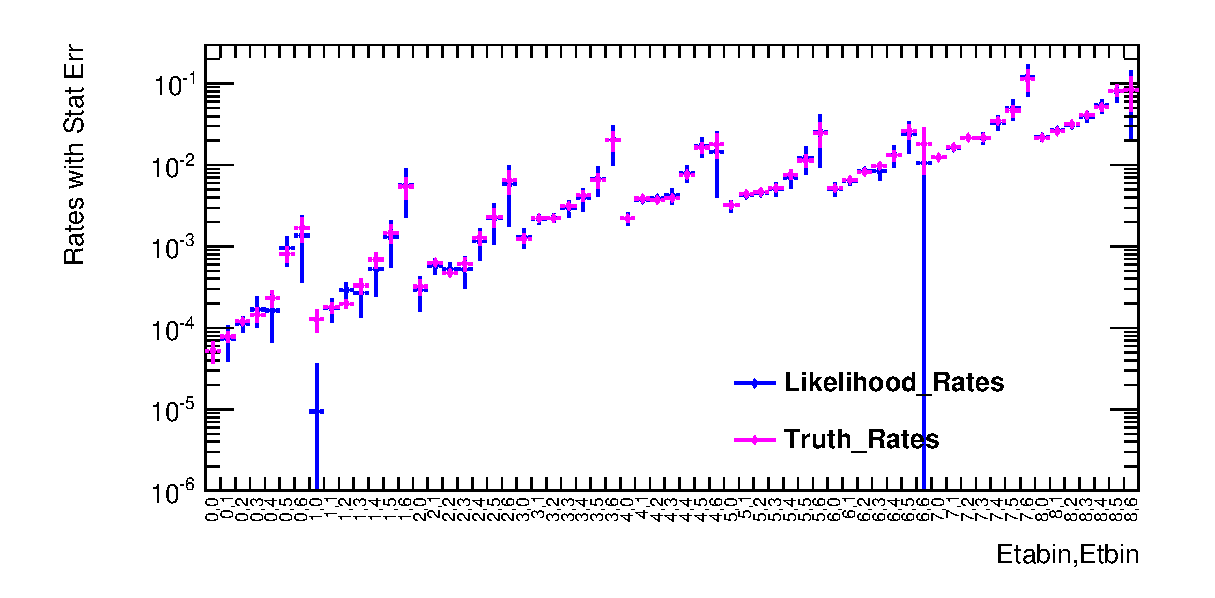
\includegraphics[width=0.8\textwidth]{figures/ChargeMisID/LL_TR_Com.eps}
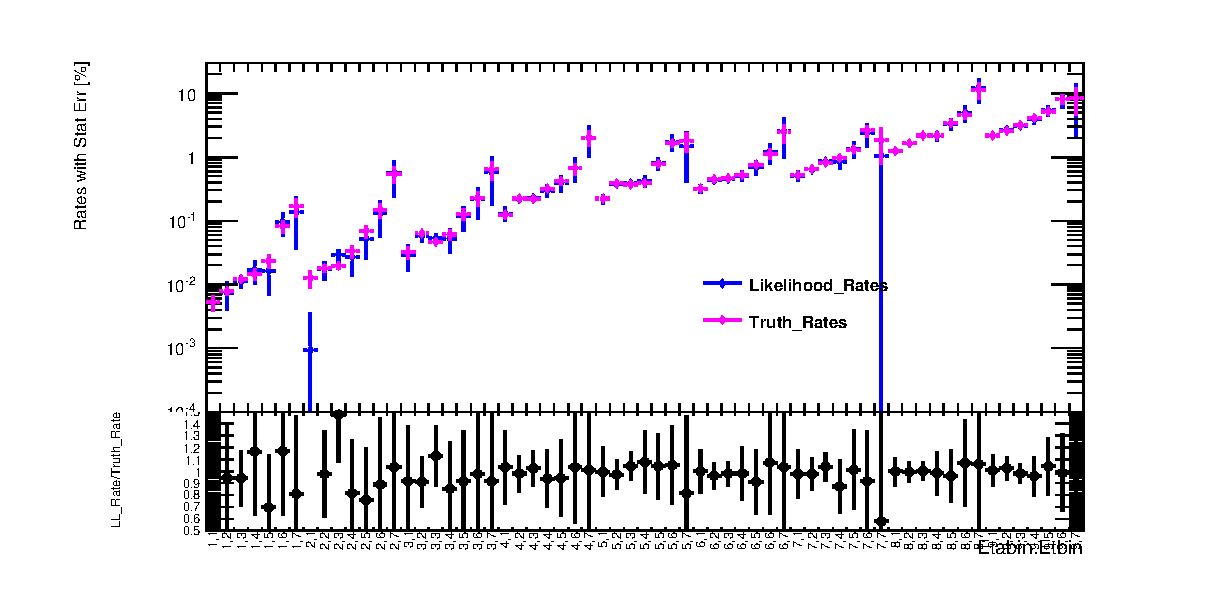
\includegraphics[width=0.8\textwidth]{figures/ChargeMisID/LL_TR_Com_new.eps}

\caption{Comparisons of the charge mis-ID rates obtained with the likelihood method and the truth method. The two sets of rates shown here were both measured with the same \Zee\ MC sample.
Statistical errors are shown. The $x$ axis label is
  the $|\eta|$, \pt\ bin index, as defined in Table~\ref{tab:Etbin and Etabin of mis-charge rate}.}
  
% This is mis-charge rate comparison between likelihood and
%   truth method considering statistic errors. The two sets of rates
%   here are both measured with \Zee\ MC samples. The $x$ axis label is
%   the \eta, \pt\ bin index.}
\label{fig:LL_Truth_Comparison}
\end{figure}  

% Through the comparison, one can see that the rates measured with the
% likelihood method are compatible with that obtained with the truth
% method. The difference between these two sets of rates is taken into account as a systematic in the final measurement.
%

 % \subsubsection{Estimation of the charge mis-ID rates in the data}


The mis-ID rates measured in data using the likelihood method are shown in Figure~\ref{fig:LL_Rates_Egamma}.

% The likelihood method is then applied in the data to measure the charge mis-ID rates.
%  % using the skimmed data from Egamma stream.
% % in Egamma stream we measure the data-driven rates with
% % (\texttt{user.along528.data12\_8TeV.period*.physics\_EGamma.PhysCont.NTUP\_SMWWW.SMN2N\_2\\Lep\_v1\_EXT0}
% % where * is A,B,C,D,E,G,H,I,J,L. These samples are slimmed with loose
% % di-lepton requirement, the di-lepton slim require there are at least 2
% % tagged high \pt\ leptons where tagged high \pt\ means Electron/Muon
% % satisfies any object quality requirement (loose, medium or tight for
% % muons and loose++,\\medium++,tight++,
% % veryLooseLL,looseLL,mediumLL,tightLL, or veryTightLL for electrons)
% % and has a pt of at least 10 GeV.).
%
% They are measured using the same selection described above. This estimation is used as the central value for the charge mis-ID rates measurement. Figure~\ref{fig:LL_Rates_Egamma}, show the central value of the rate and their statistical error as a function of the $|\eta|$ and \pt\ bin index defined in Table~\ref{tab:Etbin and Etabin of mis-charge rate}.

% They are shown as a function of the \eta and \pt\ bin index defined in Table~\ref{tab:Etbin and Etabin of mis-charge rate}, in Figure~\ref{fig:LL_Rates_Egamma}.


\begin{figure}[htp]
\centering
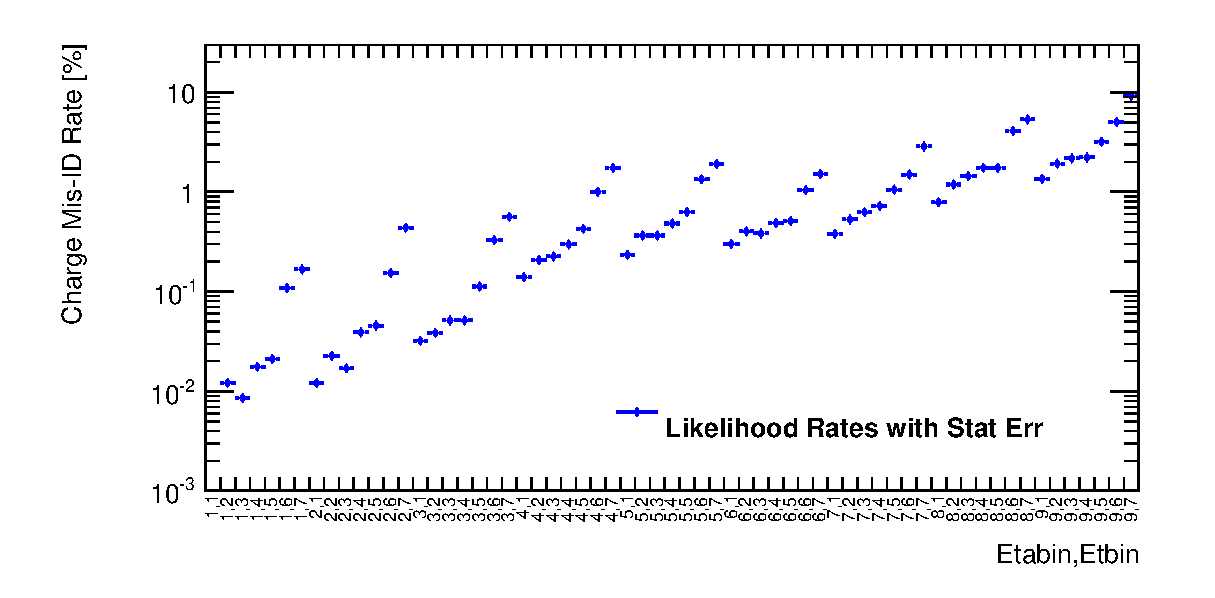
\includegraphics[width=0.8\textwidth]{figures/ChargeMisID/Egamma_LLB_new.eps}
\caption{Electron charge mis-ID rates obtained from data with the likelihood method. Statistical errors are shown. The $x$ axis label is
  the $|\eta|$, \pt\ bin index, as defined in Table~\ref{tab:Etbin and Etabin of mis-charge rate}.}

% This is electron mis-charge rates measured from data with likelihood method and its statistic errors. Label on x axis is \eta, \pt\ bin indices.}
\label{fig:LL_Rates_Egamma}
\end{figure}


 \subsubsection{Systematic effect on charge mis-ID rates due to background contamination}

The contamination of non-$Z\rightarrow{}ee$ processes in the previous selection is taken into account as a systematic.

In order to study this effect, a template fit approach is used. The signal template is obtained from the same MC simulation sample used above, while the background template is obtained from a looser data selection enriched in background events. Due to statistic constraints the background template is obtained in each $|\eta|$ bins, but the $\pt$ bins are grouped together. The event selection for the background template request the presence of a good isolated electron as defined in Section~\ref{sec:Object_selection}, and a second electron failing the tight++ identification cut. 

The two templates are then used on the invariant mass distribution of the electron pairs, in each $\pt$ and $|\eta|$ bins to determine the background contribution, subtract it and recompute the rate by maximizing the likelihood defined in Eq.~(\ref{eq:lnL_chargeMisID}). The difference between this new set of rates and the central value is then taken as a systematic uncertainty on the method, and are summarized in Table~\ref{tab:Charge_MisID_Bkg_Sys}. Further details on this method are also provided in Appendix~\ref{sec:appendix_chargeMisID}.

% The uncertainty due to the background contamination is summarized in Table~\ref{tab:Bkg Sys}.

% We estimate the background effect with
% coarser binning and include the shift in mischarge rate in the
% systematics.


%  We apply the likelihood method and event selection mentioned before
%  to data and we get the data-driven electron mis-charge rates, but
%  the rates are measured from data so there will be background events
%  remaining in the selected events. We use those rates directly
%  measured from data as central values and then subtract the
%  background contribution in the rates, we can calculate another set
%  of likelihood rates using the events without background, we may
%  call those rates clean rates. The difference between central values
%  and clean rates is the background systematic.



\begin{table}
\footnotesize
\centering
\begin{tabular}{c|c|c|c|c|c|c|c|c|c}
  \hline
  \backslashbox{\pt[\GeV]}{$|$\eta$|$} &[0,0.8] &[0.8,1.15] &[1.15,1.60] &[1.60,1.80] &[1.80,2.0] &[2.0,2.20] &[2.20,2.30] &[2.30,2.40] &[2.40,2.50] \\ 
  \hline
  [15,30] &8.85 &5.63 &5.75 &5.85 &5.79 &5.64 &5.64 &5.68 &5.49 \\
  \hline
  [30,40] &5.73 &5.71 &5.83 &5.97 &5.75 &5.78 &5.72 &5.81 &5.59 \\
  \hline
  [40,50] &5.76 &5.69 &5.71 &5.71 &5.65 &5.71 &5.62 &5.71 &5.62 \\
  \hline
  [50,60] &5.74 &5.55 &5.64 &5.53 &5.61 &5.65 &5.41 &5.49 &5.65 \\
  \hline
  [60,80] &5.77 &5.57 &5.71 &5.99 &5.59 &5.66 &5.35 &5.53 &5.41 \\
  \hline
  [80,120] &5.79 &5.63 &5.73 &5.71 &5.74 &5.77 &5.36 &5.74 &5.89 \\
  \hline
  [120,1000] &5.76 &5.71 &5.54 &5.76 &5.52 &5.61 &5.73 &5.98 &6.14  \\
  \hline
\end{tabular}
\caption{Systematic uncertainties on the central value charge mis-ID rates expressed in percent. These uncertainties were obtained considering the impact of the background contamination in the selection.}
% Numbers here are background systematics over central values
%   in percent.}
\label{tab:Charge_MisID_Bkg_Sys}
\end{table} 
 


\subsubsection{Final rates}

The rates with the final errors used in the analysis are shown in Figure~\ref{fig:ChargeMisID_truthRate_finalFig}. The total systematic uncertainty is obtained doing a quadratic sum of the error obtained comparing the MC likelihood method and the truth method, shown in Table~\ref{tab:MCLLTruthSys}, and the error obtained considering the background contamination in the selection. The rates are also given in Table~\ref{tab:LL_finalRates}.

 \begin{figure}[htp]
 \centering
 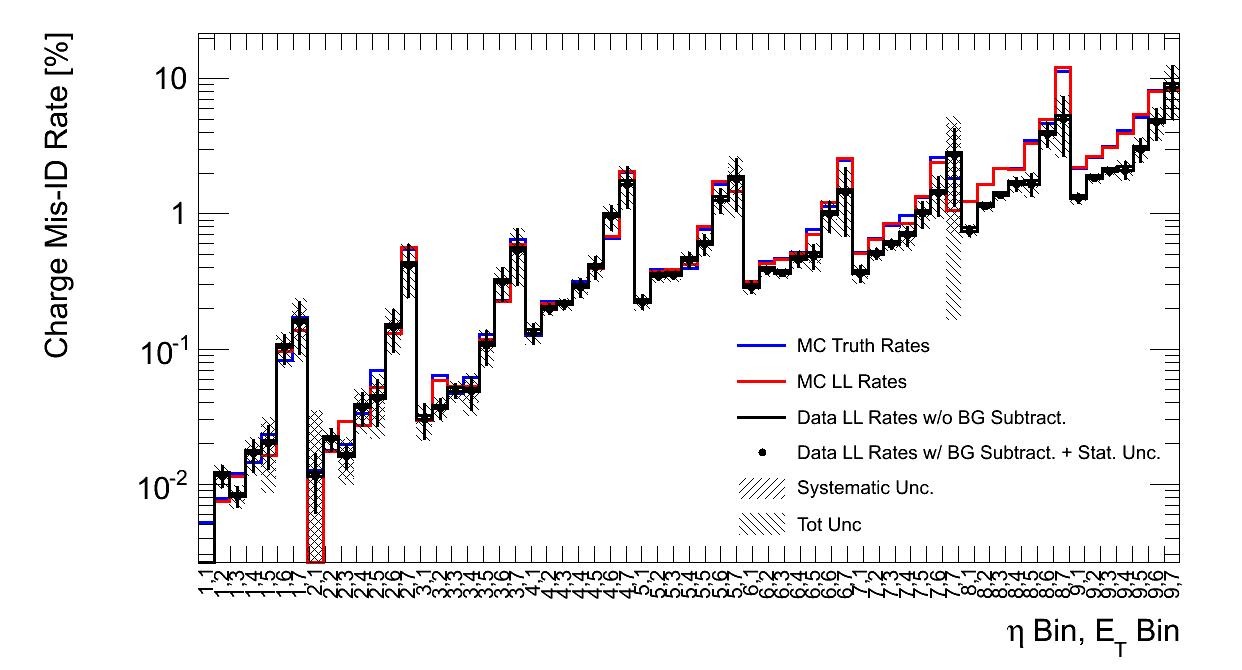
\includegraphics[width=0.8\textwidth]{figures/ChargeMisID/Validation_ChargeMisIDRates_PTvsEta_FinalRateWithSys.png}
 \caption{Electron charge mis-ID rates obtained from data with the likelihood method. All the errors are now shown. The $x$ axis label is
  the $|\eta|$, \pt\ bin index, as defined in Table~\ref{tab:Etbin and Etabin of mis-charge rate}.}
 \label{fig:ChargeMisID_truthRate_finalFig}
 \end{figure}

\begin{table}
\footnotesize
\centering
\begin{tabular}{c|c|c|c|c|c|c|c|c|c}
  \hline
  \backslashbox{\pt[\GeV]}{$|$\eta$|$} &[0,0.8] &[0.8,1.15] &[1.15,1.60] &[1.60,1.80] &[1.80,2.0] &[2.0,2.20] &[2.20,2.30] &[2.30,2.40] &[2.40,2.50] \\
  \hline
  [15,30] & $> 100$ & $> 100$ &9.24 &3.12 &0.70 &0.05 &2.27 &0.25 &0.80 \\
  \hline
  [30,40] & 5.98 &2.58 &9.91 &2.14 &2.97 &3.84 &2.51 &0.63 &2.44\\
  \hline
  [40,50] & 6.22 &32.26 &11.36 &2.19 &4.12 &2.17 &3.52 &0.43 &2.13 \\
  \hline
  [50,60] & 14.22 &22.92 &17.20 &6.72 &7.13 &2.08 &14.80 &1.75 &4.52 \\
  \hline
  [60,80] & 43.45 &32.03 &9.39 &6.14 &3.93 &9.86 &1.19 &4.22 &3.84 \\
  \hline
  [80,120] & 14.59 &12.57 &2.51 &3.14 &4.73 &6.90 &9.40 &6.40 &1.34 \\
  \hline
  [120,1000] & 23.46 &3.02 &9.53 &1.02 &22.98 &3.17 &73.12 &5.61 &3.31 \\
  \hline
\end{tabular}
\caption{The absolute value of the difference between the charge mis-identification rates derived in MC using the truth method and using the likelihood method.  Numbers
are shown as a percent of the MC likelihood method.  These are transported to the likelihood rates in data and used as a systematic. }
\label{tab:MCLLTruthSys}
\end{table}



\begin{table}
\footnotesize
\centering
\begin{tabular}{c|c|c|c|c|c|c|c|c|c}
  \hline
  \backslashbox{\pt[\GeV]}{$|$\eta$|$} &[0,0.8] &[0.8,1.15] &[1.15,1.60] &[1.60,1.80] &[1.80,2.0] &[2.0,2.20] &[2.20,2.30] &[2.30,2.40] &[2.40,2.50] \\
  \hline
  $ \times 10^{}$
  [15,30] &$1.7370\times 10^{-11}$ &$9.4036\times 10^{-6}$ &0.0003 &0.0013 &0.0022 &0.0032 &0.0051 &0.0124 &0.0219\\
  \hline
  [30,40] &$7.4276\times 10^{-5}$ &0.0002 &0.0006 &0.0022 &0.0038 &0.0043 &0.0064 &0.0165 &0.0268 \\
  \hline
  [40,50] &0.0001 &0.0003 &0.0005 &0.0023 &0.0039 &0.0046 &0.0085 &0.0218 &0.0311 \\
  \hline
  [50,60] &0.0002 &0.0003 &0.0005 &0.0030 &0.0042 &0.0051 &0.0085 &0.0213 &0.0394 \\
  \hline
  [60,80] &0.0002 &0.0005 &0.0012 &0.0040 &0.0080 &0.0070 &0.0134 &0.0332 &0.0540 \\
  \hline
  [80,120] &0.0009 &0.0013 &0.0023 &0.0068 &0.0172 &0.0122 &0.0239 &0.0497 &0.0810 \\
  \hline
  [120,1000] &0.0014 &0.0056 &0.0059 &0.0204 &0.0147 &0.0255 &0.0106 &0.1208 &0.0820  \\
  \hline
\end{tabular}
\caption{Electron charge mis-ID rates, obtained with the likelihood method on the data.}
\label{tab:LL_finalRates}
\end{table}




Although the likelihood method, which is used to determined the rates from the data, was validated in MC using the truth method, it is quite important to validate the rates as much as possible, and to verify that if there are remaining differences they are covered within the systematic uncertainties that were assigned.

%As already stated, the charge mis-ID rates are particularly important for the determination of the $WZ$ and $ZZ$ background contamination in the 0SFOS region. Therefore two more tests are conducted to test their validity.

We performed a test to recompute the charge mis-ID rates using the truth method and a $WZ$ MC sample, and compare these new rates to the old one obtained with the $Z\to{}ee$ events. In principle, the charge mis-ID is mostly due to detector effects, and it is therefore not expected to see any differences using one physics process or another one, as long as the GEANT4 geometry of the detector that was used to generate the events is the same. To perform this study, given the lower statistic available in the $WZ$ MC sample a different binning is used, it is summarized in Table~\ref{tab:Etbin and Etabin of mis-charge rate for WZ comparisons}. The new rates obtained are compared in Figure~\ref{fig:ChargeMisID_truthRate_Zee_WZ}. In this figure only the statistical error of each measurement is shown. A very good agreement between the two sets of rates is observed.



\begin{table}[htp]
\centering

\begin{tabular}{c|c||c|c}
	 \hline
	  $|\eta|$ bins & $|\eta|$ bin index   & \pt\ bins [\GeV] & \pt\ bin index \\
 	 \hline
	  $[0, 1.15]   $   & 0 	   &  $[15, 40]$ & 0 \\
	  $[1.15, 1.8] $   & 1 	   &  $[40, 60]$ & 1 \\
	  $[1.8, 2.2] $   & 2	   &  $[60, 100]$ & 2 \\
	  $[2.2, 2.5] $   & 3 	   &  $[100, 1000]$ & 3 \\

  \hline
\end{tabular}
\caption{The $|\eta|$ and \pt\ bins used for the comparison of mischarge
  rate obtained with MC $Z\to{}ee$ sample and MC $WZ$ sample. The bin index used in the 1D figures~\ref{fig:ChargeMisID_truthRate_Zee_WZ} are given.}
\label{tab:Etbin and Etabin of mis-charge rate for WZ comparisons}
\end{table}



 \begin{figure}[htp]
 \centering
 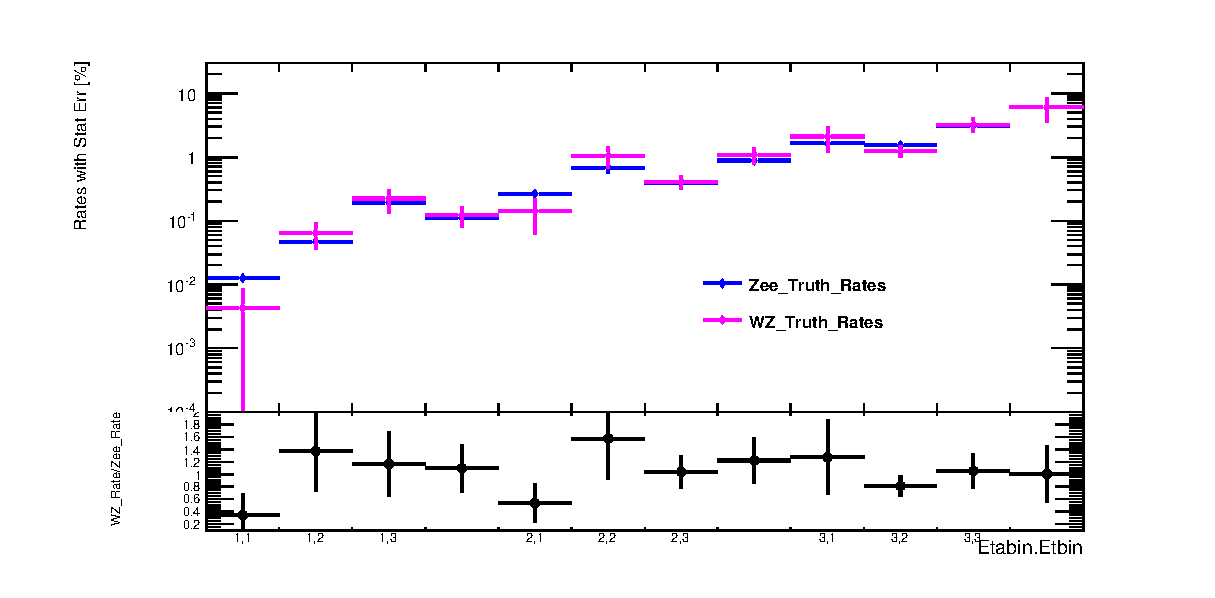
\includegraphics[width=0.8\textwidth]{figures/ChargeMisID/Validation_ChargeMisIDRates_PTvsEta_CompareSSRate.eps}
 \caption{Electron charge mis-ID rates obtained from MC $Z\to{}ee$ with the likelihood method are compared with rates obtained using the truth method in a MC $WZ$ sample. Errors shown here are purely statistics. The $x$ axis label is
  the $|\eta|$, \pt\ bin index, as defined in Table~\ref{tab:Etbin and Etabin of mis-charge rate for WZ comparisons}.}
 \label{fig:ChargeMisID_truthRate_Zee_WZ}
 \end{figure}


\subsubsection{Application and validation of rates}
As already stated, the charge mis-ID rates are primarily important for the determination of the $WZ$ and $ZZ$ background contamination in the 0SFOS region. 
Once derived, the rates are applied to $WZ$ and $ZZ$ MC samples based on whether or not a charge flip could cause the event to appear in the 0 SFOS region.  
In particular, the following di-boson decays are considered:
\begin{itemize}
\item $WZ\rightarrow e^{\pm}\nu~ e^{+}e^{-}$
\item $WZ\rightarrow \mu^{\pm}\nu~ e^{+}e^{-}$
\item $WZ\rightarrow \tau^{\pm}\nu~ e^{+}e^{-}$
\item $ZZ\rightarrow e^{+}e^{-}~e^{+}e^{-}$
\item $ZZ\rightarrow \mu^{+}\mu^{-}~ e^{+}e^{-}$
\end{itemize}
No other decay channels are considered.  These all share in common that they have at least one electron-positron pair.  
Except for the $WZ\rightarrow \tau^{\pm}\nu~e^{+}e^{-}$ decay channel, decay channels with tau leptons are not considered
because they are suppressed by the tau branching fraction and are considered to be negligible.

The charge mis-identification rates are then applied to these channels on an event-by-event basis as follows.
For each event that is processed, its decay channel is identified at truth level. Each reconstructed lepton
is examined  and assigned a rate, or a probability to charge flip, based on its reconstructed $\pt$ and $\eta$ values.
The probability for a charge flip to occur in an event is then approximately the sum of rates for the individual electrons:
\begin{equation}
\textrm{Probability of Charge Mis-Identification in Event} = \sum_{i \in \textrm{Electrons}}  \textrm{Rate}(\pt^i,\eta^i) + \textrm{Higher Order Terms}
\end{equation}
Higher order terms where multiple electrons are charge mis-identified is small and considered to be negligible.
We are only concerned with the probability that a charge flip results in the event falling into the 0 SFOS region. 
Consider a step function, $\Theta(e)$, defined for an individual event:
\[
\Theta(e) = 
\begin{cases}
\hfill 1 \hfill & \text{if flipping charge of $e$ classifies event as 0 SFOS} \\
\hfill 0 \hfill & \text{if flipping charge of $e$ does NOT classify event as 0 SFOS}\\
\end{cases}
\]
Then the probability that a charge mis-identification occurs and results in the event falling in the 0 SFOS region is:
\begin{equation}
\textrm{Probability that event is classified as 0 SFOS} = \sum_{i \in \textrm{Electrons}}  \textrm{Rate}(\pt^i,\eta^i)\Theta(i) + \textrm{Higher Order Terms}
\end{equation}
Again, we ignore the case where multiple electrons have their charge mis-identified.  
This probability is then used as an event by event weight. 



Once the weight has been determined, we then artificially flip the charge of one of the electrons/positrons in the event.
If there is only one electron in the event that will lead the event to fall in the 0 SFOS region, its charge is flipped
and one proceeds to the next event.  If there are multiple electrons in the event, however, there is an ambiguity that must be resolved
about which electron's charge should be flipped. One must then be careful in this case to not introduce any bias.
We decided to choose a procedure where we pick a single electron from the event at random based on the charge flip rates
of the individual electrons. Thus, for an individual electron in an event, the probability that it is chosen to have its charge
flipped is:
\begin{equation}
\textrm{Probability that $e$ has charge flipped} = \textrm{Rate}(\pt^e,\eta^e)\Theta(e)~/\sum_{i \in \textrm{Electrons}} \textrm{Rate}(\pt^i,\eta^i)\Theta(i)
\end{equation}

Consider an example 
where the event under consideration comes from the decay $WZ\rightarrow e^{+}\nu e^{+}e^{-}$. Assume all three charged leptons pass reconstruction and are selected then label them as: $e^{+}_1~e^{+}_2e^{-}_3$. In this case,
the only way that this event could be classified as 0 SFOS when flipping the charge of only one electron/positron is to flip the charge of the electron.
Thus, $\Theta(e^{+}_1)=\Theta(e^{+}_2)=0$ and $\Theta(e^{-}_3)=1$.  The event weight will then be equal to the rate of charge mis-identification for  $e^{-}_3$ and it
will have it's charge flipped to be positive.

Now consider an example of an event with the decay of $ZZ\rightarrow \mu^{+}\mu^{-}~ e^{+}e^{-}$.
If all four leptons are reconstructed and selected, the event will not be considered at all in the three lepton selection of this analysis, so consider the 
case where the $\mu^{+}$ is not selected leaving three leptons labeled as: $\mu^{-}_1 e^{+}_2 e^{-}_3$.  The probability for the muon to charge flip
is negligible which leaves the electron and the positron. Flipping the charge of either one at a time will result in the event being classified as 0 SFOS.  Thus, in
this case $\Theta(\mu^{-}_1)=0$ and $\Theta(e^{+}_2)=\Theta(e^{-}_3)=1$. The event weight will then be the sum of the rates for $e^{+}_2$ and $e^{-}_3$.
The probability that the electron has its charge flipped is then $\frac{\textrm{Rate}(e^{-}_3) }{ \textrm{Rate}(e^{+}_2)+ \textrm{Rate}(e^{-}_3)}$ and similarly for the positron.

This procedure has been validated on the $WZ$ and $ZZ$ samples by comparing the predictions taken directly from MC to the predictions re-weighted in the 0 SFOS signal region using the procedure just described. This is done in Figure~\ref{fig:ChargeMisID_Validation_WZ} for the $WZ$ samples and on Figure~\ref{fig:ChargeMisID_Validation_ZZ} for the $ZZ$ samples. It can be seen the agreement in the shape looks good for all the distributions. An offset between the two distributions is observed. This difference is covered partially by the systematic uncertainties of the method.  Any remaining difference could be expected from the difference in rates observed at high $\eta$ and high $E_{T}$ as seen in Fig.~\ref{fig:ChargeMisID_truthRate_finalFig} and serves as justification for using the data-driven method.

There is no special treatment of the charge mis-identification contribution to other background contributions in the 0 SFOS region or to any contributions to the 
1 and 2 SFOS signal regions, including di-boson processes, as the effect is expected to be very small.  Any charge mis-identification events are thus taken directly 
from MC in this case.


 \begin{figure}[htp]
 \centering
 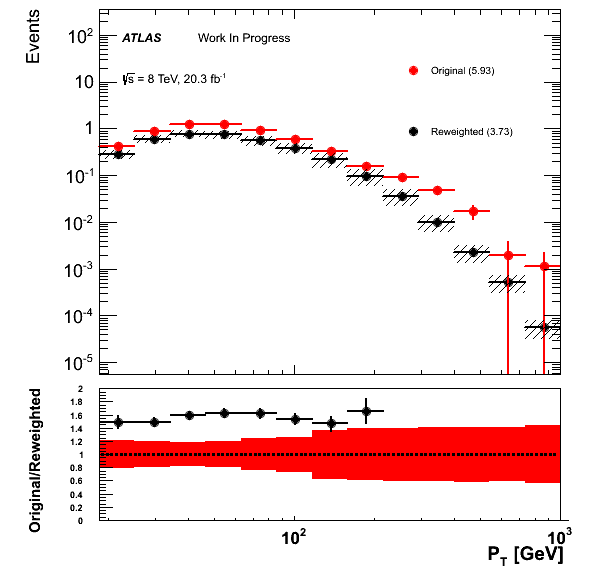
\includegraphics[width=0.4\textwidth]{figures/ChargeMisID/Validation_ChargeMisIDRates_WZ_PTLepton.png}
 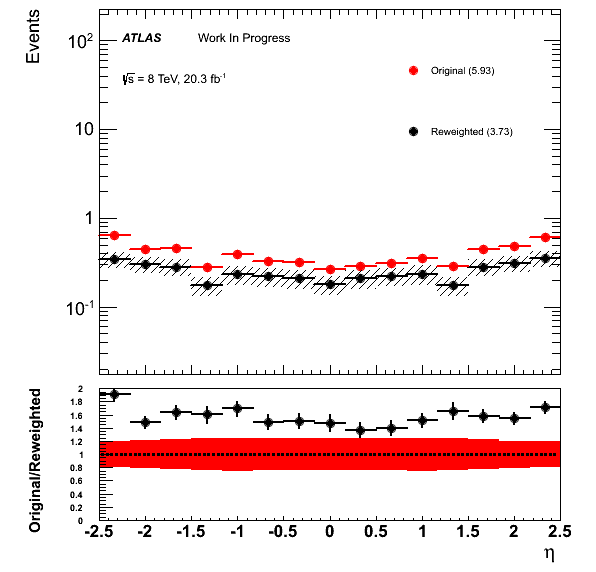
\includegraphics[width=0.4\textwidth]{figures/ChargeMisID/Validation_ChargeMisIDRates_WZ_EtaLepton.png}
 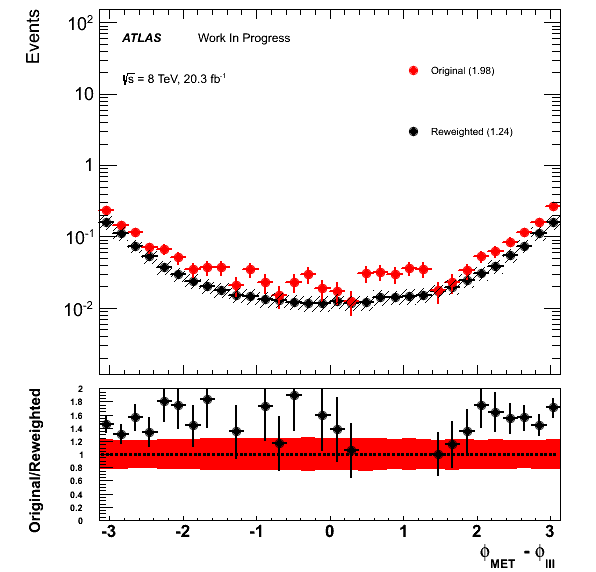
\includegraphics[width=0.4\textwidth]{figures/ChargeMisID/Validation_ChargeMisIDRates_WZ_DeltaPhi.png}
 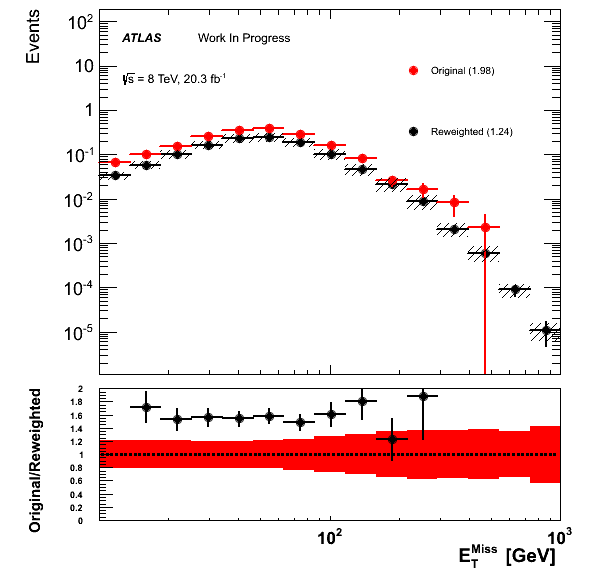
\includegraphics[width=0.4\textwidth]{figures/ChargeMisID/Validation_ChargeMisIDRates_WZ_MET.png}
 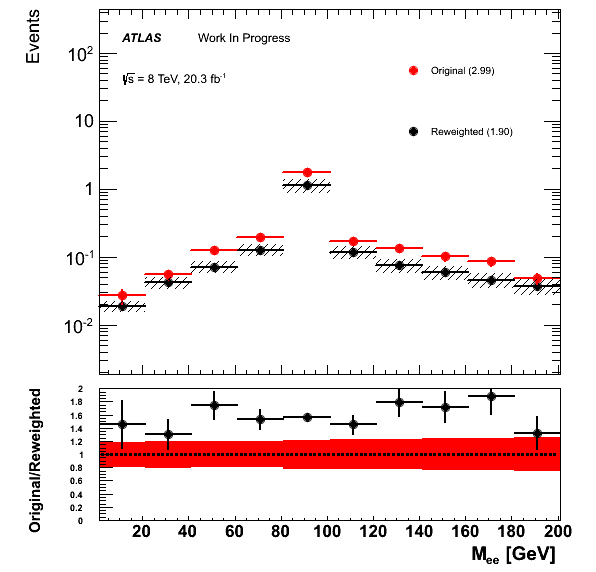
\includegraphics[width=0.4\textwidth]{figures/ChargeMisID/Validation_ChargeMisIDRates_WZ_Mee.png}
 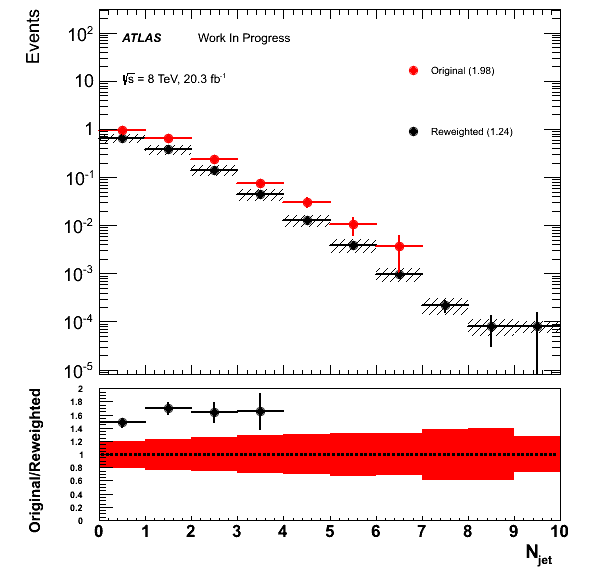
\includegraphics[width=0.4\textwidth]{figures/ChargeMisID/Validation_ChargeMisIDRates_WZ_JetMultiplicity.png}

 \caption{Validation of the charge mis-ID rates comparing MC $WZ\rightarrow \ell ee$ ($\ell=e,\mu$) samples re-weighted with the charge mis-ID rates measured in the MC $Z\to{}ee$ 
 sample to the original MC predictions. Distribution of lepton $p_{T}$, $\eta$, $\Delta \phi(3l,E_{T}^{Miss})$,\met{}, Same-sign di-electron invariant mass, and jet multiplicity.}
 \label{fig:ChargeMisID_Validation_WZ}
 \end{figure}
 
 
 \begin{figure}[htp]
 \centering
 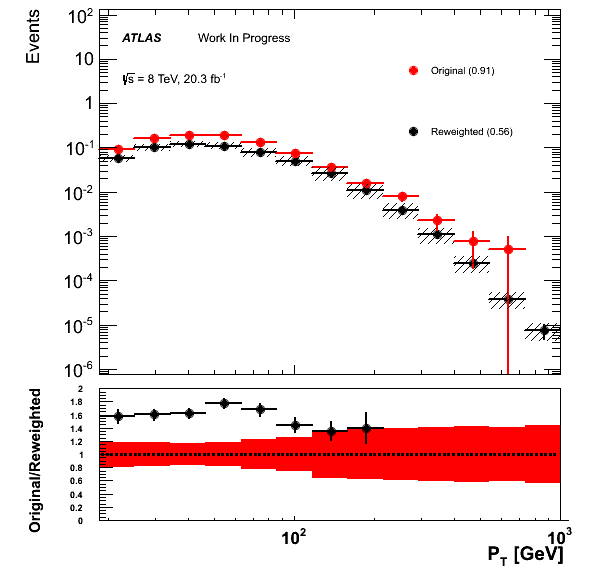
\includegraphics[width=0.4\textwidth]{figures/ChargeMisID/Validation_ChargeMisIDRates_ZZ_PTLepton.png}
 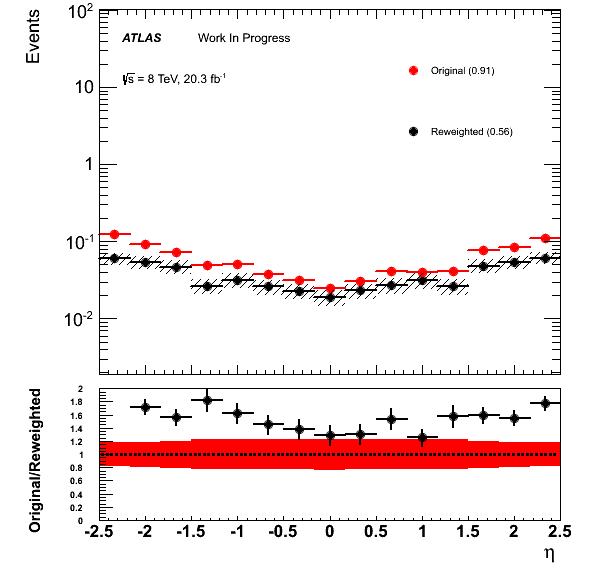
\includegraphics[width=0.4\textwidth]{figures/ChargeMisID/Validation_ChargeMisIDRates_ZZ_EtaLepton.png}
 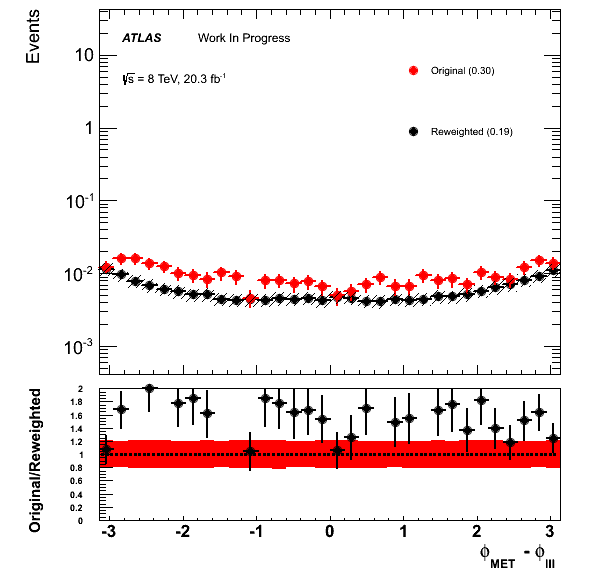
\includegraphics[width=0.4\textwidth]{figures/ChargeMisID/Validation_ChargeMisIDRates_ZZ_DeltaPhi.png}
 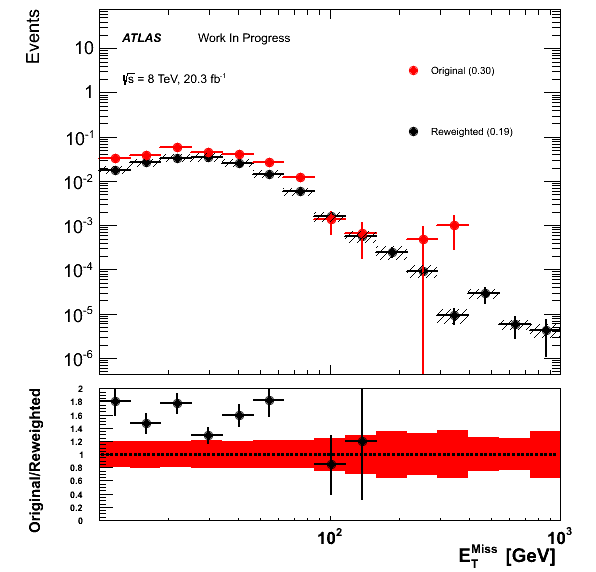
\includegraphics[width=0.4\textwidth]{figures/ChargeMisID/Validation_ChargeMisIDRates_ZZ_MET.png}
 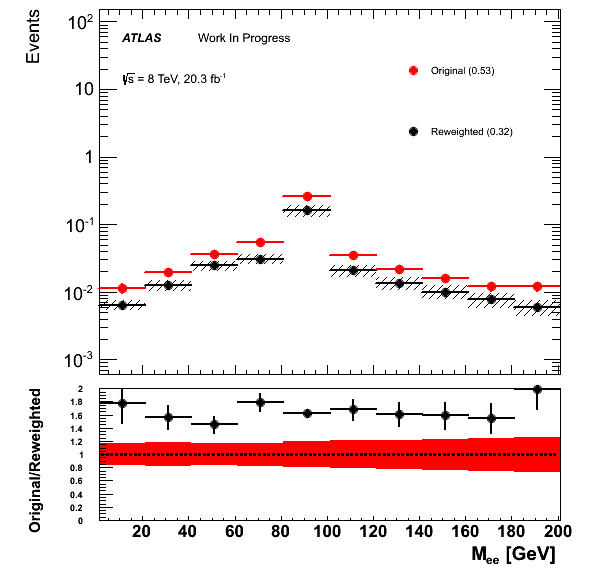
\includegraphics[width=0.4\textwidth]{figures/ChargeMisID/Validation_ChargeMisIDRates_ZZ_Mee.png}
 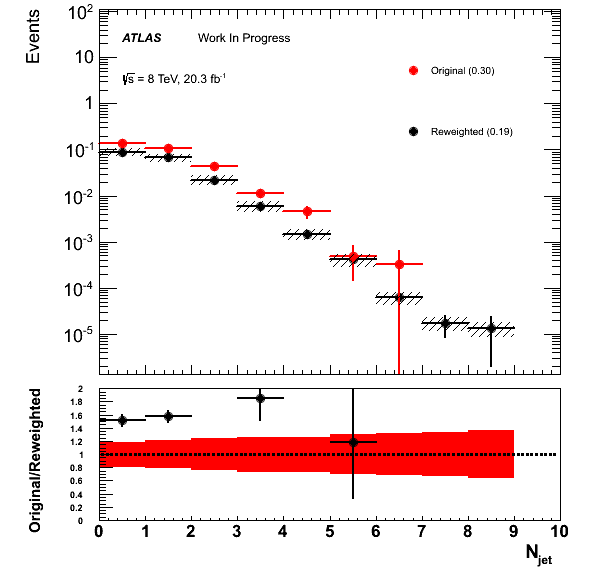
\includegraphics[width=0.4\textwidth]{figures/ChargeMisID/Validation_ChargeMisIDRates_ZZ_JetMultiplicity.png}

 \caption{Validation of the charge mis-ID rates comparing MC $ZZ\rightarrow \ell \ell ee$ ($\ell=e,\mu$) samples re-weighted with the charge mis-ID rates measured in the MC $Z\to{}ee$ 
 sample to the original MC predictions. Distribution of lepton $p_{T}$, $\eta$, $\Delta \phi(3l,E_{T}^{Miss})$,\met{}, Same-sign di-electron invariant mass, and jet multiplicity.}
 \label{fig:ChargeMisID_Validation_ZZ}
 \end{figure}






